\documentclass[]{standalone}

\usepackage{../lenses}

\begin{document}
 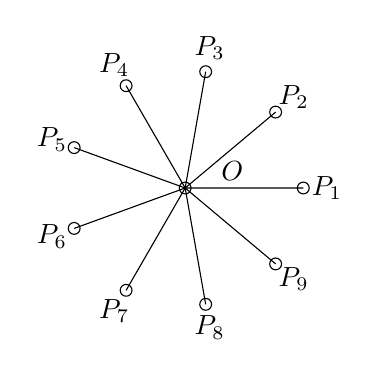
\begin{tikzpicture}
  \begin{scope}[scale=1.5]
   \draw(0,0) circle(0.05) ++(0.4,0.14) node{$O$};
   \foreach \x in {1,2,3,4,5,6,7,8,9} {
    \pgfmathsetmacro{\n}{40*(\x-1)}
    \draw(0,0) -- (\n:1) circle(0.05) ++(\n:0.2) node{$P_\x$};
   }
  \end{scope}
 \end{tikzpicture}
\end{document}